\documentclass[12pt,a4paper]{article}
\usepackage[top=2cm,bottom=2cm,left=2cm,right=2cm]{geometry}
\usepackage[dvipsnames]{xcolor}
\usepackage{graphicx}
\usepackage{polski}
\usepackage{amsmath}
\usepackage{amsfonts}
\usepackage{makecell}
\usepackage{color}
\usepackage{float}
\usepackage{parskip}
\usepackage{tabularray}
\usepackage{caption}
\usepackage{subcaption}
\usepackage{minted}
\usepackage[shortlabels]{enumitem}
\usepackage{url}
\usepackage{hyperref}

\graphicspath{{./images/}}
\DeclareCaptionJustification{centering}{\centering}
\captionsetup{justification=centering}

\author{Rafał Chrzanowski, Maria Gajek, Maja Szczypka}
\title{Symulacja krakowskiej sieci tramwajowej \\ \vspace{0.25cm} \Large Raport końcowy}


\begin{document}
    \maketitle

    \newpage

    \tableofcontents

    \newpage

    \section{Wstęp}
        Celem projektu było stworzenie symulatora działania sieci tramwajowej w Krakowie. W projekcie zostały uwzględnione linie tramwajowe dzienne, których ruch przedstawiony został na mapie Krakowa. Ruch tramwajów odbywa się według rzeczywistego rozkładu jazdy uzyskanym ze strony internetowej Zarządu Transportu Publicznego w Krakowie. Symulowane tramwaje unikają kolizji między sobą oraz zatrzymują się na wskazanych przystankach.

    \section{Podobne problemy spotykane w literaturze}
        Organizacja i modelowanie transportu publicznego jest problemem z którym zmierza się każde większe miasto. Okazuje się, że transport szynowy jest popularną i ważną częścią ekosystemów transportowych w miastach. Aby adekwatnie rozplanować i stworzyć infrastrukturę w danym mieście, należy uwzględnić przede wszystkim ilość mieszkańców oraz ich lokalne zapotrzebowanie.

        Problem ten został poruszony w artykule Chia Len Chen \cite{china_tram} o integracji pojazdów szynowych w komunikacji miejskiej w Chinach. Ważnym z perspektywy miast w Chinach jest administracyjny podział tego rodzaju komunikacji i dopasowanie go do warunków terenowych i zapotrzebowania. Zbadano i oszacowano zapotrzebowanie w określonych regionach, przedstawiono różne projekty modernizacji i przebudowy istniejących linii. Symulowano projekty nowych linii i przystanków tramwajowych w procesie ich tworzenia. Zwrócono uwagę na fakt iż tramwaje i lekka kolej szynowa w Europie jest klasyfikowana jako ten sam rodzaj transportu. Modelowanie różni się więc w zależności od regionu.

        Problem modernizacji i usprawnienia połączeń samego Krakowa również jest poruszany w artykułach naukowych. W artykule \textit{Integration of the Urban Public Transportation System with the Application of Traffic Simulation} \cite{krk_sim}. Tu skupiono się na porównaniu istniejącego już systemu komunikacji z teoretycznym nowym systemem wymagającym dużego nakładu finansowego w celu modernizacji wcześniejszego. Symulowano i porównywano proponowane czasy przejazdu ilości przesiadek i obłożenie każdego z rodzajów transportu w Krakowie.

        Projekty zawierające symulacje nie opierają się jednak tylko na przewidywaniu rozwijania obecnych systemów. Poruszają one również problematykę użycia obecnej infrastruktury do nowych celów. Tematem zajmuję się artykuł \textit{Simulation Model for Operational Planning of City Cargo Transportation by Trams in Conditions of Stochastic Demand}\cite{poz_sim}.  Na przykładzie innego polskiego miasta z rozwiniętą infrastrukturą tramwajową - Poznania - stworzono symulacje i propozycje wykorzystania jej do przewożenia towarów dotychczas dostarczanych transportem samochodowym.

        Wyżej wspomniane modele są konkretnymi przykładami problemu który nawet w przypadkach teoretycznych jest dosyć złożony. Propozycje tworzenia modeli nie tylko tych kolejowych dobrze opisuje \textit{Simulation models for public transportation: a state-of-the-art review} \cite{sim_models}. Opisany model symulacji agentowej jest bliski projektowi opisanemu w tym raporcie i jest bazą dla wielu innych.

        Praktyczna strona problemu transportu tramwajowego zaowocowała stworzeniem uniwersalnego narzędzia do jego rozwiązania. TRAMS\cite{TRAMS} jest narzędziem pozwalającym na przetestowanie zmian w zarządzaniu ruchem przed ich wprowadzeniem. Autorzy stworzyli projekt z myślą o operatorach i administracji zarządu transportu publicznego w różnych miastach. TRAMS podobnie jak projekt któremu dedykowany jest ten raport na podstawie danych o lokalizacji przystanków, dostępnych połączeniach torowych, przystankach końcowych i wielu innych tworzy model, animuje go i dodatkowo przeprowadza analizę przewidując zachowanie danego ustawienia sieci tramwajowej.

    \section{Problemy napotkane w projekcie}
        \subsection{Pozyskanie danych o rozkładach jazdy}
            Informacje zawarte w rozkładach jazdy nie pozwalają na proste wyznaczenie każdego z przejazdów tramwajów. Spowodowało to problemy z interpretowaniem wczytanych danych za pomocą skryptu. Część linii nie funkcjonuje w weekendy lub święta, na niektórych występują kursy wariantowe, jeszcze inne kończą swoje kursy po północy. Wzięcie wszystkich tych sytuacji pod uwagę nie było proste, ale okazało się być możliwe.

        \subsection{Wyznaczenie dokładnych tras tramwajów}
            Najprostszym sposobem na pokazanie stanów pośrednich między przystankami jest poruszanie się danego tramwaju wzdłuż linii prostej wyznaczonej przez te dwa przystanki. Takie rozwiązanie okazało się być jednak mało satysfakcjonujące oraz utrudniające realizację unikania kolizji między tramwajami. W celu pozbycia się tego problemu, udało się wyznaczyć faktyczne trasy tramwajów wykorzystując dane OpenStreetMap.

        \subsection {Integracja danych}
            W celu wizualizacji przejazdów na prawdziwej mapie Krakowa konieczne było połączenie odpowiednich przystanków z bazy danych wraz z ich odpowiednikami na mapie. Przeszkodą okazało się nazewnictwo przystanków między nimi. Często napotykano błędy takie jak różnica w nazwie, niepoprawna numeracja lub nawet jej brak i niesprecyzowany numer przystanku końcowego w rozkładach. Aby zapobiec tym problemom, wykonano poprawki w danych oraz zaimplementowano sposoby na manualną interwencję wykonującego skrypt.

        \subsection{Zapobieganie kolizjom}
            Po udanej implementacji poruszania się tramwajów wzdłuż torowiska zauważyliśmy, że dość często występują między nimi kolizje. Rozważyliśmy kilka możliwych implementacji zapobiegania kolizji, z których najbardziej optymalne okazało się odpytywanie wyroczni, czy na podstawie przyszłej trasy tramwaj może wykonać ruch. Pozostałe rozważane sposoby wielokrotnie generowały trudne do usunięcia zakleszczenia albo były bardzo kosztowne obliczeniowo. Oczywiście nadal możliwe jest wygenerowanie zakleszczenia stosując odpowiednie parametry symulacji, ale ich domyślne wartości powinny zapobiegać większości z nich.

    \newpage

    \section{Zbiór danych}
        Przed uruchomieniem symulacji, powinna ona posiadać dane dotyczące lokalizacji przystanków, przejazdów każdego z tramwajów oraz tras między przystankami. Zgromadzone dane zostają zapisane w bazie danych SQLite:

        \begin{figure}[H]
            \centering
            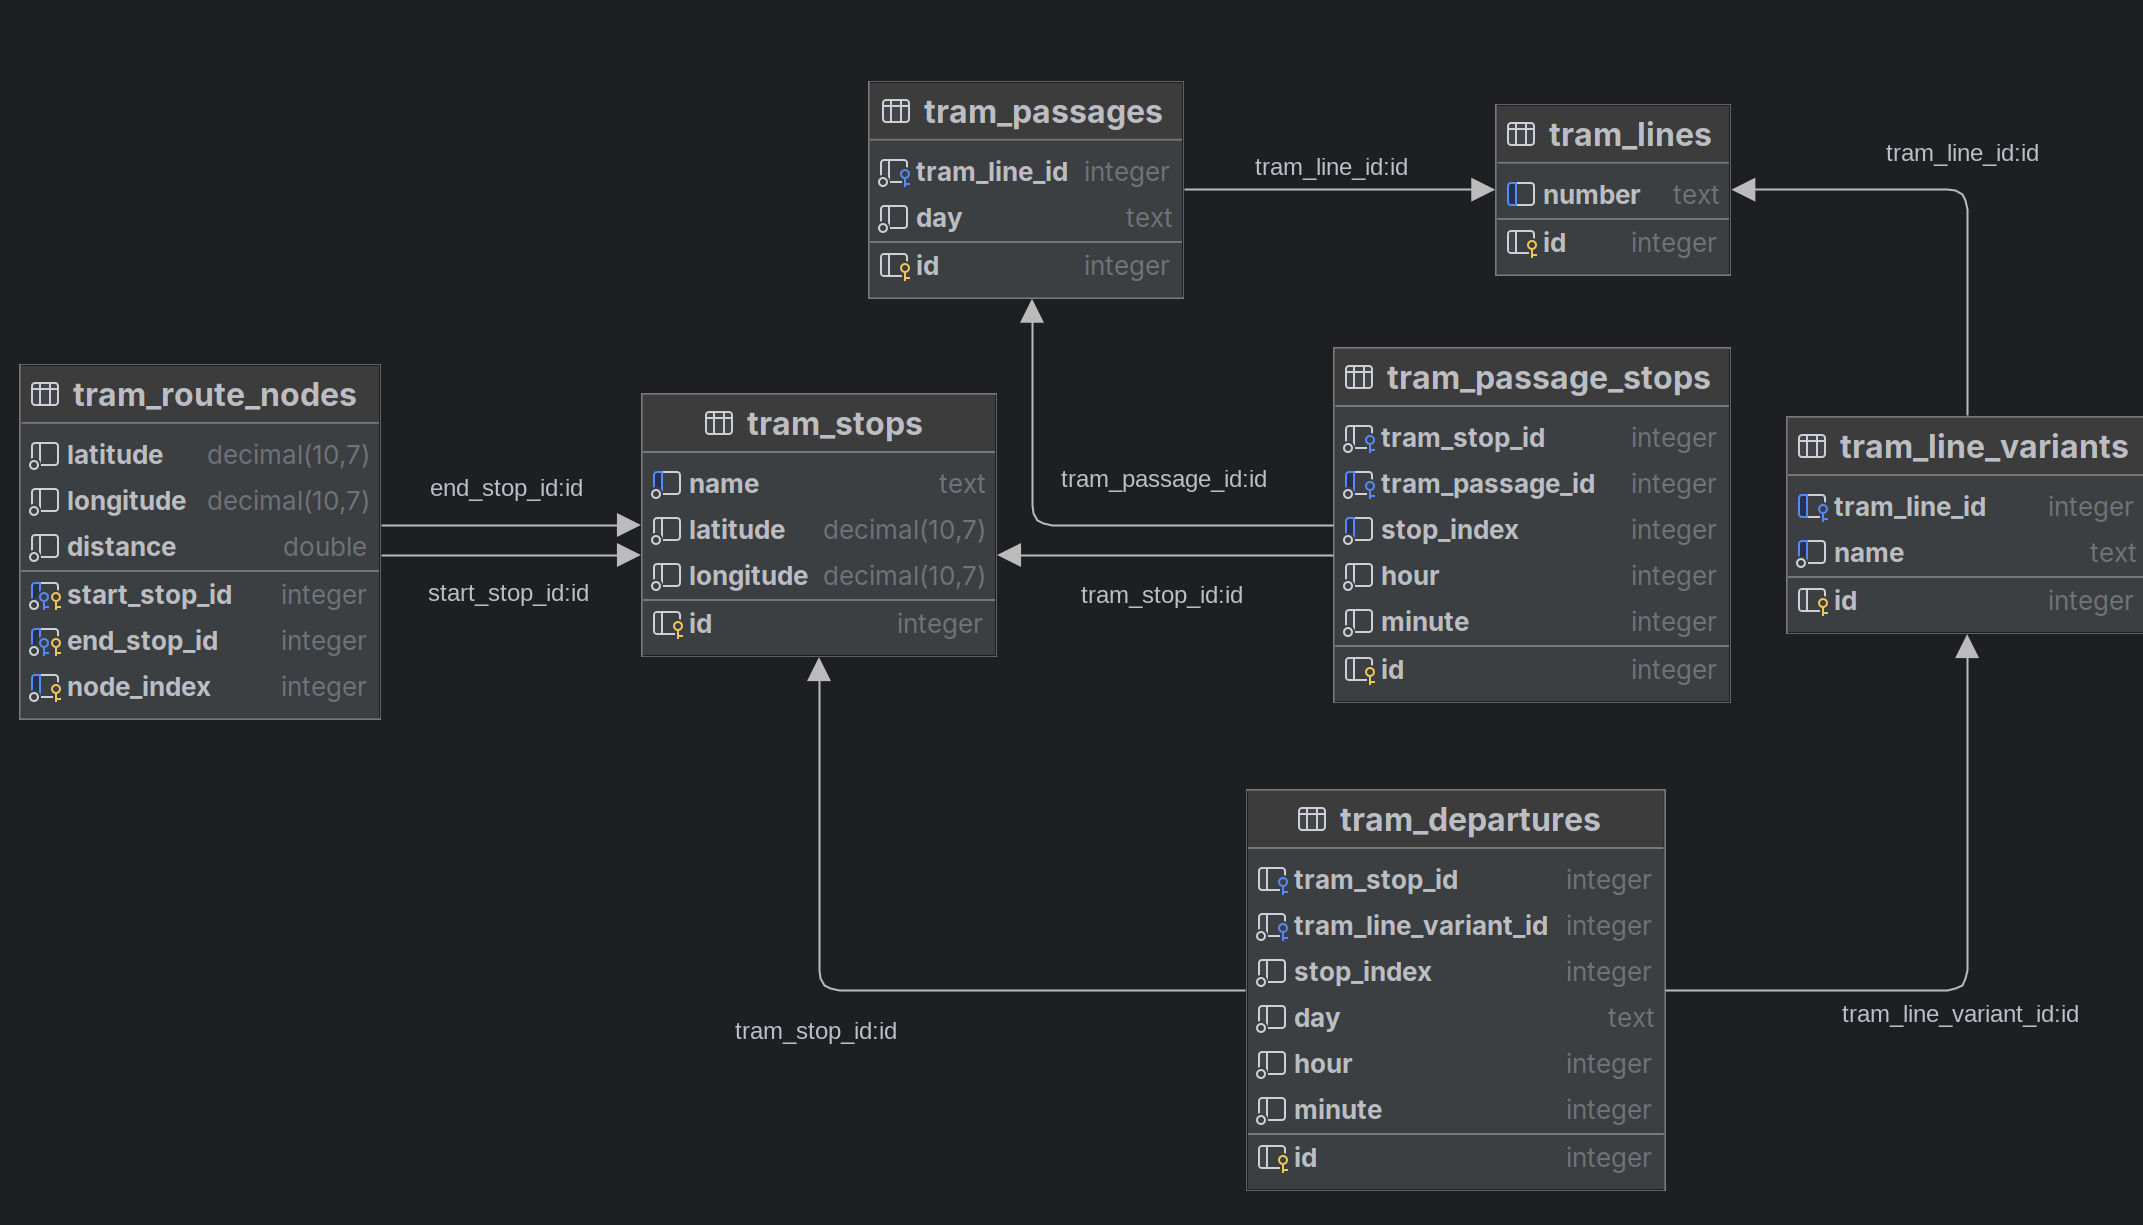
\includegraphics[width=\textwidth]{database-diagram.png}
            \caption{Schemat bazy danych}
        \end{figure}

        \subsection{Przystanki tramwajowe}
            W celu zebrania danych dotyczących nazw i pozycji przystanków tramwajowych w Krakowie, posłużono się danymi z OpenStreetMap. Pozyskano je za pomocą biblioteki \texttt{overpy}\cite{overpy}, wykorzystującej narzędzie Overpass turbo, poprzez wykonanie poniższej kwerendy, której wynik zapisano w tabeli \texttt{tram\_stops}:

\begin{verbatim}
[out:json];
area["name"="Kraków"]->.search_area;
node["tram"="yes"]["railway"="tram_stop"](area.search_area);
out;
\end{verbatim}

            W czasie zbierania informacji dotyczących przystanków, wykryto kilka błędów i rozbieżności w danych OSM. Wykonane zostały zatem poniższe poprawki:
            \begin{itemize}
                \item \url{https://www.openstreetmap.org/changeset/150757574}
                \item \url{https://www.openstreetmap.org/changeset/150848336}
                \item \url{https://www.openstreetmap.org/changeset/150853365}
                \item \url{https://www.openstreetmap.org/changeset/150893766}
                \item \url{https://www.openstreetmap.org/changeset/150939752}
                \item \url{https://www.openstreetmap.org/changeset/150979527}
                \item \url{https://www.openstreetmap.org/changeset/150999378}
            \end{itemize}

        \subsection{Czasy odjazdów tramwajów}
            W celu zebrania informacji o czasach odjazdów tramwajów, wykonano skrypt w języku Python wykorzystujący narzędzie \texttt{StatefulBrowser} z biblioteki \texttt{mechanicalsoup}\cite{mechanicalsoup}. Na stronie z rozkładami jazdy znajdujemy listę wszystkich działających linii tramwajowych, dla każdej z nich znajdujemy ich warianty, następnie dla każdego wariantu pobieramy listę przystanków z którego się składa dany wariant i dla każdego takiego przystanku pobieramy czasy odjazdów w zależności od typu dnia.

            Informacje na temat linii tramwajowych przechowujemy w tabeli \texttt{tram\_lines}. Dane dotyczące wariantów linii tramwajowej przechowujemy w tabeli \texttt{tram\_line\_variants}. Czasy odjazdów tramwajów z danego przystanku przechowujemy w tabeli \texttt{tram\_departures}.

            W przypadku nierozpoznania nazwy przystanku przez skrypt, pyta on użytkownika o to jakim znanym mu przystankiem powinien go zastąpić, takimi przystankami są np. przystanki wokół Placu Centralnego im. Ronalda Reagana, których nazwy w danych OSM różnią się od tych prezentowanych w rozkładzie jazdy.

            Ponadto w przypadku napotkania przystanku końcowego, wymagane jest potwierdzenie użytkownika czy wskazany przez skrypt przystanek zgadza się z rzeczywistością. Przypadki, w których wymagana jest zmiana proponowanego przystanku, zdarzają się np. jeśli tramwaj kończy swój bieg na pętli Krowodrza Górka P+R, gdzie faktycznym przystankiem końcowym jest Krowodrza Górka P+R 01, a skrypt proponuje przystanek znajdujący się w innym miejscu.

        \subsection{Przejazdy tramwajów}
            Korzystając z informacji dotyczących rozkładu jazdy, wyznaczono przejazdy każdego z tramwajów, czyli listy kolejnych przystanków wraz z czasami odjazdu. Proces ten jest o tyle skomplikowany, że nie wszystkie kursy tramwajów zaczynają się na przystanku początkowym linii, nie wszystkie kończą się na przystanku końcowym oraz niektóre z nich kończą się po północy. Po przeanalizowaniu rozkładów jazdy wariantów linii 1, 4, 20 i 50, został wymyślony algorytm odporny na wszystkie napotkane powyżej problemy:

\begin{minted}{python}
def _get_variant_passages(self, tram_line_id: int, variant_id: int,
                          day: DayType) -> list[TramPassage]:
    def add_departure(departure: Departure):
        tram_passage.add_stop(departure)
        departure_passage[departure] = tram_passage

    departures, stop_index_departures = self._get_departures(variant_id, day)

    passages: list[TramPassage] = []
    departure_passage: dict[Departure, TramPassage] = {}

    # Some lines don't have any passages on saturdays and holidays
    if not departures:
        return passages

    highest_stop_index = max(stop_index_departures.keys())
    for end_departure in filter(lambda x: x not in departure_passage,
                                departures):
        tram_passage = TramPassage(tram_line_id, day)
        passages.append(tram_passage)

        if end_departure.stop_index < highest_stop_index:
            new_first_departure = self._get_new_first_departure(end_departure)
            departures.append(new_first_departure)
            add_departure(new_first_departure)

        previous_stop = end_departure
        for stop_index in filter(
            lambda x: x <= end_departure.stop_index,
            sorted(stop_index_departures.keys(), reverse=True)
        ):
            next_stop = min(
                stop_index_departures[stop_index],
                key=lambda x: x.time_distance_between(previous_stop)
            )

            if next_stop.time_distance_between(previous_stop) >= 60:
                break
            elif next_stop in departure_passage:
                later_passage = departure_passage[next_stop]
                for _ in range(later_passage.get_departure_index(next_stop),
                               len(later_passage)):
                    del departure_passage[
                        later_passage.reverse_stop_sequence.pop()
                    ]

            tram_passage.add_stop(next_stop)
            departure_passage[next_stop] = tram_passage
            previous_stop = next_stop

    return passages
\end{minted}

            Informacje dotyczące każdego przejazdu tramwajów przechowywane są w tabeli \texttt{tram\_passages}. Dane dotyczące kolejnych przystanków przejazdu tramwaju przechowujemy w tabeli \linebreak \texttt{tram\_passage\_stops}.

        \subsection{Trasy między przystankami}
            Aby tramwaje w czasie wykonania symulacji poruszały się wzdłuż torowiska, należy wyznaczyć listy współrzędnych kolejnych węzłów ich trasy. Dodatkowo dla każdego węzła wyznaczono jego odległość od punktu startowego wykorzystując bibliotekę \texttt{geopy}\cite{geopy}, ponieważ określenie odległości na kuli posługując się prostokątnym układem współrzędnych jest znacznie nietrywialne. Informacja, między którymi przystankami należy wyznaczyć trasy, została uzyskana poprzez wykonanie poniższej kwerendy:

\begin{minted}{sql}
SELECT DISTINCT
    tram_passage_stops.tram_stop_id AS start_stop_id,
    TPS.tram_stop_id AS end_stop_id
FROM tram_passage_stops
    JOIN tram_passage_stops TPS ON
        tram_passage_stops.tram_passage_id = TPS.tram_passage_id
WHERE tram_passage_stops.stop_index = TPS.stop_index - 1
\end{minted}

            W celu uzyskania informacji dotyczących przebiegu torowisk tramwajowych, wykonano kwerendę wykorzystującą bibliotekę \texttt{overpy}:

\begin{verbatim}
[out:json];
area["name"="Kraków"]->.search_area;
(
    way["railway"="tram"]["oneway"="yes"](area.search_area);
    >;
);
out geom;
\end{verbatim}

            Za pomocą zgromadzonych powyżej danych, wykonano graf skierowany ważony, w którym węzłami były węzły z danych OSM będącymi punktami z których składają się łamane reprezentujące torowisko, a krawędziami były połączenia tych węzłów o wagach równych ich odległości między nimi. Na takim grafie dla każdej pary przystanków wykonano zmodyfikowany algorytm Dijkstry, który oprócz znalezienia optymalnej odległości między przystankami określał także optymalną trasę:

\begin{minted}{python}
def route_between_nodes(self, start_node_id: int, end_node_id: int):
    """
        This method implements a modified version of Dijkstra's algorithm.
        In this implementation it is possible to not only find the shortest
        distance between two nodes, but also the shortest path between them.
        The implementation also does not search the entire graph, but stops
        when no further improvement is possible.
    """

    priority_queue: PriorityQueue[tuple[float, GraphNode]] = PriorityQueue()
    parents: dict[int, GraphNode | None] = {}
    distances: dict[int, float] = defaultdict(lambda: float("inf"))

    priority_queue.put((0, self.graph[start_node_id]))
    parents[start_node_id] = None
    distances[start_node_id] = 0

    while priority_queue.not_empty:
        current_distance, root = priority_queue.get()

        if current_distance > distances[end_node_id]:
            break

        for node in self.graph[root.id].edges:
            new_distance = distances[root.id] + root.distance_to(node)

            if distances[node.id] > new_distance:
                distances[node.id] = new_distance
                parents[node.id] = root
                priority_queue.put((distances[node.id], node))

    result: list[tuple[GraphNode, float]] = []

    node = self.graph[end_node_id]
    while node is not None:
        result.append((node, distances[node.id]))
        node = parents[node.id]

    result.reverse()

    return result
\end{minted}

            Otrzymaną w ten sposób trasę zapisywano do tabeli \texttt{tram\_route\_nodes}.

    \section{Implementacja symulacji}
        Symulacja została zaimplementowana jako aplikacja webowa, której serwer napisany w języku Python wykorzystujący framework \texttt{Flask}\cite{flask} służy do przesyłania danych z utworzonej wcześniej bazy danych do klienta, a klient jest napisany przy użyciu języka TypeScript, frameworka Vue.js i biblioteki \texttt{Vuetify}\cite{vuetify}. Wizualizację mapy oraz wskazywanie pozycji, kierunku oraz linii tramwajów zrealizowano wykorzystując bibliotekę \texttt{Leaflet}\cite{leaflet}.

        \subsection{Synchronizacja czasu}
            Poruszanie się tramwajów w symulacji odbywa się w sposób zsynchronizowany. Przy każdej zmianie aktualnego czasu symulacji, na każdej instancji tramwaju wywoływana jest metoda \texttt{move}, która obsługuje pojawianie się tramwaju na mapie, jego znikanie z mapy, czekanie na przystanku oraz zmienianie jego pozycji. Po przemieszczeniu wszystkich tramwajów zwiększany jest czas symulacji o jedną sekundę za pomocą metody \texttt{advance} klasy \texttt{Time}.

        \subsection{Ruch tramwajów}
            W celu sprawdzenia, czy tramwaj może się poruszyć, tramwaj wykorzystuje metodę \texttt{canAdvance} klasy \texttt{AdvancementOracle}. Metoda ta sprawdza, czy na trasie wskazanej przez parametr \texttt{checkRoute} znajduje się inny tramwaj oraz czy węzły tej trasy nie są już zablokowane. Jeśli odpowiedź wyroczni jest pozytywna, rezerwuje ona trasę dla tramwaju wskazywaną przez argument \texttt{blockRoute}.

            Tramwaj powinien pojawić się na mapie, jeśli aktualny czas jest taki sam jak czas jego pierwszego odjazdu pomniejszony o czas oczekiwania na przystanku. W takiej sytuacji tramwaj informuje wyrocznię o swoim pojawieniu się i dodaje się do mapy. Jeśli w danej chwili węzeł, na którym ma się pojawić tramwaj, jest zablokowany, wyrocznia wstrzyma ruch tramwaju do czasu aż węzeł wskazujący jego lokalizację będzie wolny.

            Jeśli tramwaj dotrze do swojego ostatniego przystanku oraz zakończy się jego postój na przystanku, informuje on wyrocznię o swoim zniknięciu, usuwa się z mapy i resetuje swój rozkład jazdy.

            Za wskazanie kolejnej pozycji tramwaju oraz jego przyszłych tras odpowiedzialna jest klasa \texttt{TramRouteIndicator}, która znając przystanek początkowy, przystanek końcowy oraz czas przejazdu między nimi, generuje kolejne pozycje tramwaju wraz z jego orientacjami. Tramwaj przy pojawianiu się oraz dojechaniu na przystanek tworzy nową instancję tej klasy i korzysta z niej za każdym razem, kiedy chce zmienić swoją pozycję.

        \subsection{Wyświetlanie tramwajów na mapie}
            Każdy tramwaj posiada swój własny marker wskazujący jego pozycję na mapie oraz orientację. Marker ten jest trójkątem równoramiennym, którego podstawa jest prostopadła do kierunku jazdy, a wektor między podstawą a przeciwległym wierzchołkiem jest zgodny z kierunkiem jazdy tramwaju. Przy wykonaniu ruchu przez tramwaj, aktualizuje on pozycję oraz orientację swojego markera. Nad każdym markerem wyświetlany jest także numer linii, której kurs wykonuje tramwaj.

    \section{Efekt końcowy}
        Symulacja w formie końcowej prezentuje się następująco:
        \begin{figure}[H]
            \centering
            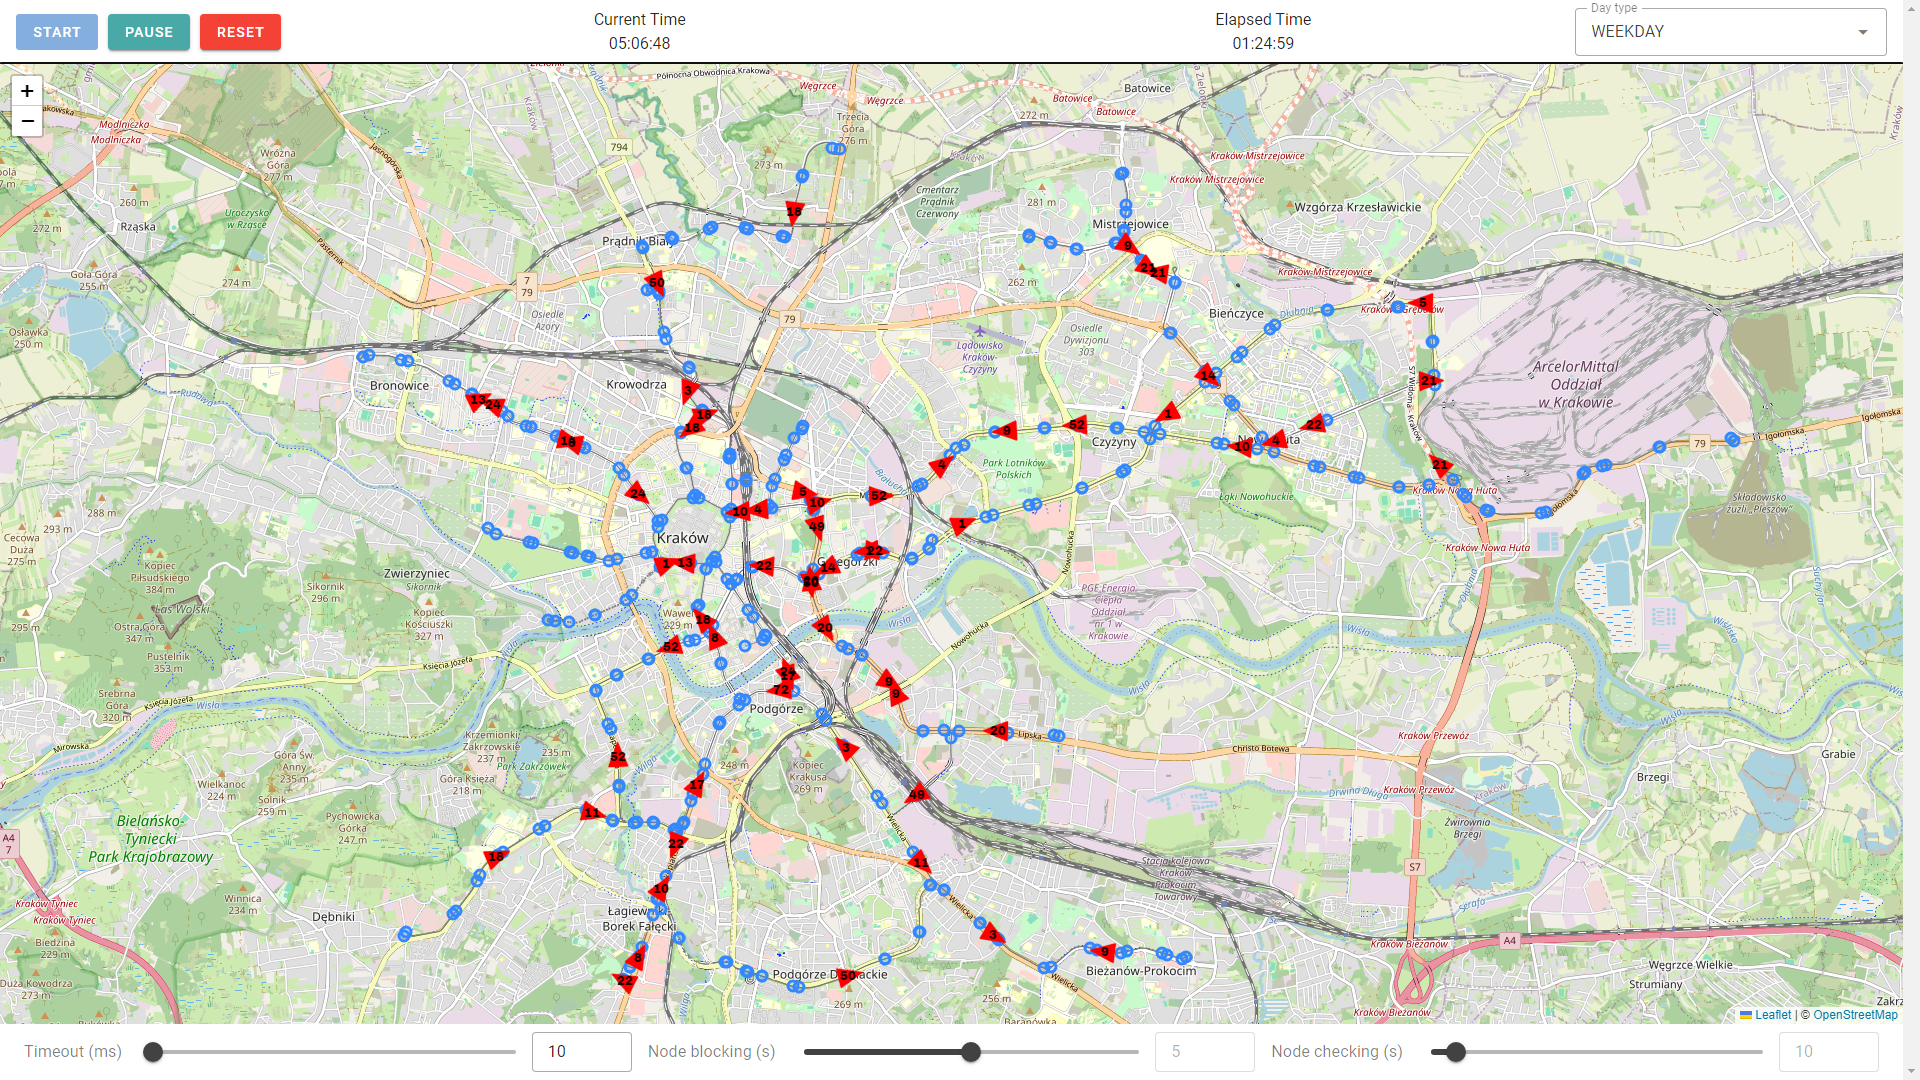
\includegraphics[width=\textwidth]{final_efect.png}
            \caption{Przykładowy wygląd działającej symulacji}
        \end{figure}

        Symulowane tramwaje zatrzymują się na przystankach, podróżują wzdłuż torowiska oraz wskazują swój kierunek. Na każdym ze wskaźników położenia tramwaju wyświetla się numer linii tramwajowej, której kurs jest wykonywany przez dany tramwaj. W czasie podróży występują opóźnienia w postaci wydłużonego czasu wymiany pasażerów, który zajmuje od 15 do 25 sekund.

        Możliwy jest wybór typu dnia, według którego realizowane będą rozkłady jazdy tramwajów. Kontrola działania symulacji odbywa się za pomocą przycisków:
        \begin{itemize}
            \item \texttt{START} odpowiadającego za rozpoczęcie jej wykonania,
            \item \texttt{PAUSE} odpowiadającego za wstrzymanie symulacji,
            \item \texttt{RESET} odpowiadającego za przywrócenie symulacji do pierwotnego stanu.
        \end{itemize}

        Symulacja za pomocą trzech suwaków pozwala na kontrolowanie parametrów symulacji, takich jak opóźnienia między kolejnymi sekundami symulacji, liczba sekund, dla których wymagana jest niezablokowana droga, by tramwaj mógł poruszać się do przodu oraz liczba sekund, którą tramwaj blokuje w celu wykonania ruchu. W celu zmiany dwóch ostatnich parametrów wymagany jest reset symulacji.

        Realizacja symulacji dostępna jest na stronie \url{https://tns.rcralph.me}.

    \section{Wyniki działania}
        Wykonaliśmy symulację dla różnych wartości parametrów \textit{Node blocking} i \textit{Node checking}. Zaobserwowaliśmy, że zwiększając wartość \textit{Node checking}, tramwaje utrzymywały większe odległości między sobą, a \textit{Node blocking} zwiększało odległość pozostałych tramwajów od skrzyżowania, przez które przejeżdża dany tramwaj. Znaleźliśmy także sytuację, w której nadal występują zakleszczenia na skrzyżowaniach.

        \begin{figure}[H]
            \centering
            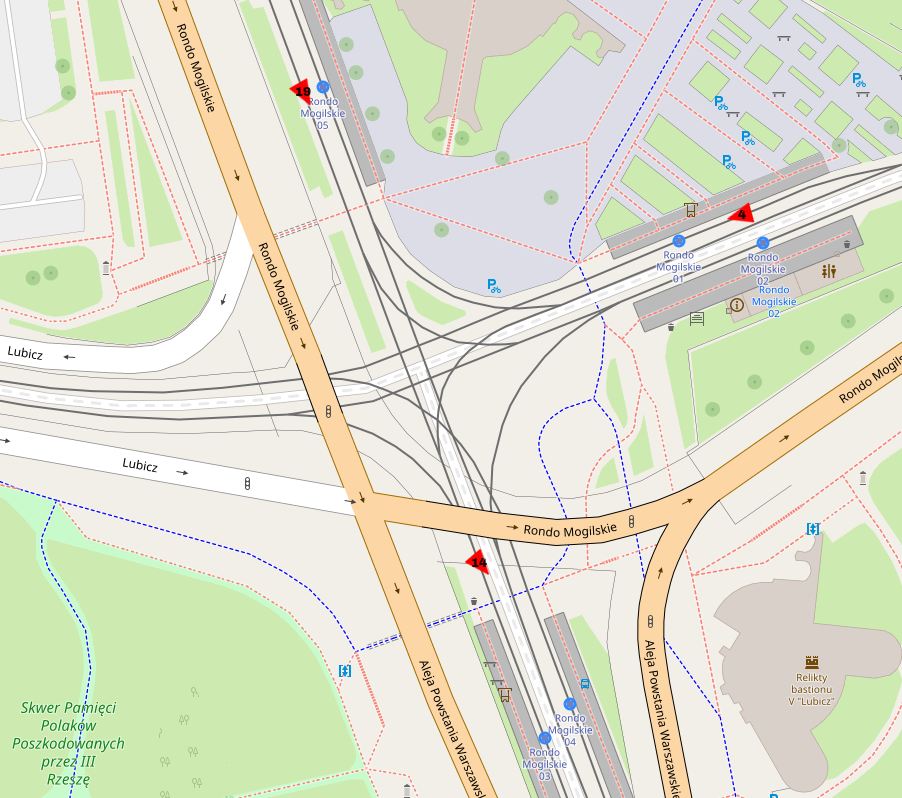
\includegraphics[width=\textwidth]{distance-5-10.png}
            \caption{Odstęp tramwajów dla parametrów \textit{Node blocking} = 5 i \textit{Node checking} = 10}
        \end{figure}

        \begin{figure}[H]
            \centering
            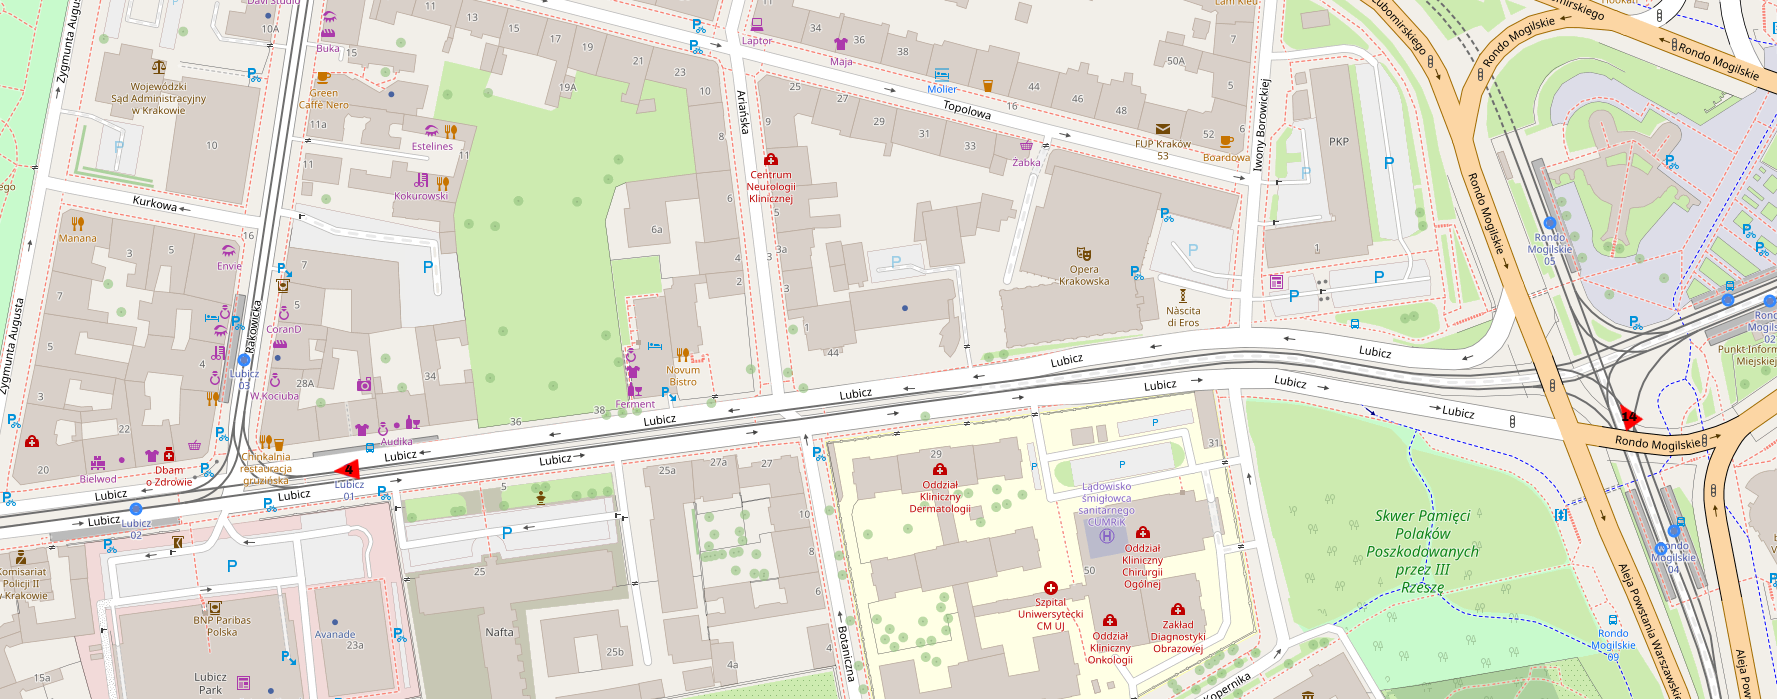
\includegraphics[width=\textwidth]{distance-5-30.png}
            \caption{Odstęp tramwajów dla parametrów \textit{Node blocking} = 5 i \textit{Node checking} = 30}
        \end{figure}

        \begin{figure}[H]
            \centering
            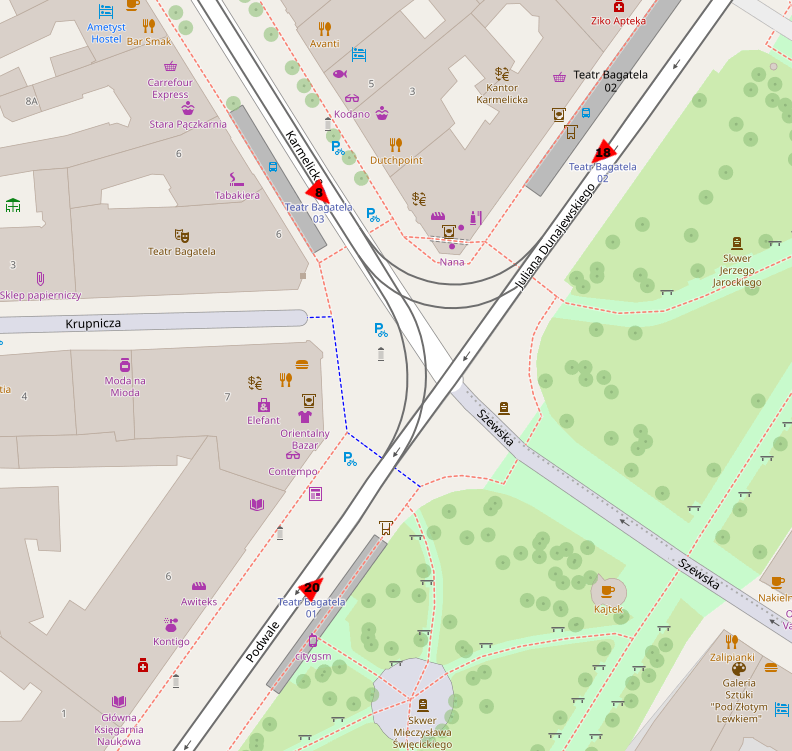
\includegraphics[width=\textwidth]{distance-20-30.png}
            \caption{Zakleszczenie tramwajów dla parametrów \textit{Node blocking} = 5 i \textit{Node checking} = 30}
        \end{figure}

    \section {Podsumowanie i wnioski}
        Projekt był ciekawym i pracochłonnym zadaniem, które pokazało wiele niewidocznych na pierwszy rzut oka aspektów związanych z modelowaniem systemów dyskretnych. Znaczna większość czasu tworzenia symulacji została poświęcona na odpowiednie zebranie i przetworzenie danych, bez których wykonanie jej nie byłoby możliwe.

        Podczas zbierania i przetwarzania danych oraz programowania symulacji została wykorzystana zdobyta wcześniej wiedza informatyczna z obszarów web scrapingu, synchronizacji wątków, algorytmów i struktur danych, web developmentu, baz danych oraz zaawansowanych technik programowania w języku Python. Może być to w pewnym sensie wstęp do projektu inżynierskiego.

        Największym problemem działania symulacji jest jej obliczeniowe obciążenie. Ponieważ do realizacji funkcji klienta wybrany został język TypeScript, jakakolwiek próba wprowadzenia wielowątkowości jest ograniczona przez jednowątkowość interpretera. Dodatkowym problemem jest spora ilość danych, których przesłanie jest wymagane do uruchomienia symulacji.

        Możliwe drogi dalszego rozwoju tego projektu zawierają usprawnienie sposobu unikania kolizji tramwajów, usprawnienie wyliczania kolejnych pozycji tramwajów z uwzględnieniem zmiennej prędkości, sygnalizacji świetlnej, stanu oraz geometrii torowiska. Możliwe jest także dodanie agentów w postaci pasażerów, którzy pojawialiby się na przystanku ze wskazaną trasą i wykorzystując tramwaje dojeżdżaliby do końca swoich tras.

    \newpage

    \begin{thebibliography}{99}
        \bibitem{TRAMS}
        \href{https://onlinelibrary.wiley.com/doi/epdf/10.1002/atr.5670190205}{TRAMS: Transit Route Animation and Modeling by Simulation, Upali Vandeboma, Anthony J. Richardson}

        \bibitem{sim_models}
        \href{https://www.sciencedirect.com/science/article/pii/S1877050922023304?ref=cra_js_challenge&fr=RR-1}{Simulation models for public transportation: a state-of-the-art review, García-Cerrud Carmen A., Flores de la Mota Idalia}

        \bibitem{krk_sim}
        \href{https://www.sciencedirect.com/science/article/pii/S2352146514001689}{Integration of the urban public transportation system with the application of traffic simulation, Katarzyna Solecka, Jacek Żak}

        \bibitem{poz_sim}
        \href{https://www.mdpi.com/1996-1073/16/10/4076}{Simulation Model for Operational Planning of City Cargo Transportation by Trams in Conditions of Stochastic Demand, Agnieszka Merkisz-Guranowska, Natalya Shramenko, Marcin Kiciński, Vladyslav Shramenko}

        \bibitem{china_tram}
        \href{https://www.itf-oecd.org/sites/default/files/docs/public-transport-integration-chinese-cities.pdf}{Modern Tram and Public Transport Integration in Chinese Cities: A case study of Suzhou, Chia-Lin Chen}

        \bibitem{mechanicalsoup}
        \href{https://mechanicalsoup.readthedocs.io/en/stable/}{MechanicalSoup}

        \bibitem{geopy}
        \href{https://geopy.readthedocs.io/en/stable/}{GeoPy}

        \bibitem{overpy}
        \href{https://pypi.org/project/overpy/}{overpy}

        \bibitem{flask}
        \href{https://flask.palletsprojects.com/en/3.0.x/}{Flask}

        \bibitem{vuetify}
        \href{https://vuetifyjs.com/en/}{Vuetify}

        \bibitem{leaflet}
        \href{https://leafletjs.com}{Leaflet}
    \end{thebibliography}
\end{document}
